%
% First sample - testing some random stuff
% !TEX program = lualatex
%
\documentclass[a5paper,ngerman,11pt]{article}
\usepackage{fontspec}
%\setmainfont[Ligatures=TeX]{Bodoni 72}
\usepackage{microtype}
\usepackage{blindtext}
\usepackage{geometry}
%\usepackage{dtklogos}
\usepackage{babel}
\usepackage{graphicx}
\usepackage{hyperref}

\hypersetup{
    pdfauthor={Thilo Mezger},
    pdfsubject={Mein Betreff},
    pdftitle={Mein Titel},
    pdfkeywords={Test, Beispiel}
}

\title{Tonio Kröger}
\author{von Thomas Mann}
\date{1921}

\begin{document}

\maketitle

\section{Erstes Kapitel}
Die Wintersonne stand nur als armer Schein, milchig und matt hinter
Wolkenschichten über der engen Stadt. Naß und zugig war's in den
giebeligen Gassen, und manchmal fiel eine Art von weichem Hagel, nicht
Eis, nicht Schnee.

Die Schule war aus. Über den gepflasterten Hof und heraus aus der
Gatterpforte strömten die Scharen der Befreiten, teilten sich und
enteilten nach rechts und links. Große Schüler hielten mit Würde ihr
Bücherpäckchen hoch gegen die linke Schulter gedrückt, indem sie mit dem
rechten Arm wider den Wind dem Mittagessen entgegen ruderten; kleines
Volk setzte sich lustig in Trab, daß der Eisbrei umherspritzte und die
Siebensachen der Wissenschaft in den Seehundsränzeln klapperten. Aber
hie und da riß alles mit frommen Augen die Mützen herunter vor dem
Wotanshut und dem Jupiterbart eines gemessen hinschreitenden
Oberlehrers . . .

»Kommst du endlich, Hans?« sagte Tonio Kröger, der lange auf dem
Fahrdamm gewartet hatte; lächelnd trat er dem Freunde entgegen, der im
Gespräch mit anderen Kameraden aus der Pforte kam und schon im Begriffe
war, mit ihnen davon zu gehen ... »Wieso?« fragte er und sah Tonio
an.... »Ja, das ist wahr! Nun gehen wir noch ein bißchen.«

Tonio verstummte, und seine Augen trübten sich. Hatte Hans es vergessen,
fiel es ihm erst jetzt wieder ein, daß sie heute mittag ein wenig
zusammen spazieren gehen wollten? Und er selbst hatte sich seit der
Verabredung beinahe unausgesetzt darauf gefreut!

\begin{center}
    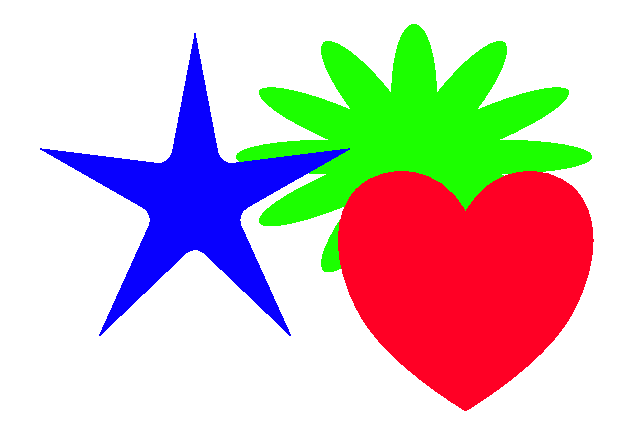
\includegraphics[width=6cm]{HerzStern.pdf}    
\end{center}

»Ja, adieu, ihr!« sagte Hans Hansen zu den Kameraden. »Dann gehe ich
noch ein bißchen mit Kröger.« -- Und die beiden wandten sich nach links,
indes die anderen nach rechts schlenderten.

Hans und Tonio hatten Zeit, nach der Schule spazieren zu gehen, weil sie
beide Häusern angehörten, in denen erst um vier Uhr zu Mittag gegessen
wurde. Ihre Väter waren große Kauf"|leute, die öffentliche Ämter
bekleideten und mächtig waren in der Stadt. Den Hansens gehörten schon
seit manchem Menschenalter die weitläufigen Holzlagerplätze drunten am
Fluß, wo gewaltige Sägemaschinen unter Fauchen und Zischen die Stämme
zerlegten. Aber Tonio war Konsul Krögers Sohn, dessen Getreidesäcke mit
dem breiten schwarzen Firmendruck man Tag für Tag durch die Straßen
kutschieren sah; und seiner Vorfahren großes altes Haus war das
herrschaftlichste der ganzen Stadt ... Beständig mußten die Freunde, der
vielen Bekannten wegen, die Mützen herunternehmen, ja, von manchen
Leuten wurden die Vierzehnjährigen zuerst gegrüßt ...

\setlength\arraycolsep{1.4pt}
\begin{equation}
    \left.
    \begin{array}{r@{\hspace{.75em}}ccrr}
        \textrm{a}) & y & = & d                     & \textrm{(konstant)}   \\[1pt]
        \textrm{b}) & y & = & cx+d                     & \textrm{(linear)}   \\
        \textrm{c}) & y & = & bx^2+cx+d                     & \textrm{(quadratisch)}   \\
    \end{array}
    \right\} \textrm{Polynome}
\end{equation}

Beide hatten die Schulmappen über die Schultern gehängt, und beide waren
sie gut und warm gekleidet; Hans in eine kurze Seemanns-Überjacke, über
welcher auf Schultern und Rücken der breite, blaue Kragen seines
Marineanzuges lag, und Tonio in einen grauen Gurtpaletot. Hans trug eine
dänische Matrosenmütze mit schwarzen Bändern, unter der ein Schopf
seines bastblonden Haares hervorquoll. Er war außerordentlich hübsch und
wohlgestaltet, breit in den Schultern und schmal in den Hüften, mit
freiliegenden und scharf blickenden stahlblauen Augen. Aber unter Tonios
runder Pelzmütze blickten aus einem brünetten und ganz südlich scharf
geschnittenen Gesicht dunkle und zart umschattete Augen mit zu schweren
Lidern träumerisch und ein wenig zaghaft hervor ... Mund und Kinn waren
ihm ungewöhnlich weich gebildet. Er ging nachlässig und ungleichmäßig,
während Hansens schlanke Beine in den schwarzen Strümpfen so elastisch
und taktfest einherschritten ...

Tonio sprach nicht. Er empfand Schmerz. Indem er seine etwas schräg
stehenden Brauen zusammenzog und die Lippen zum Pfeifen gerundet hielt,
blickte er seitwärts geneigten Kopfes ins Weite. Diese Haltung und Miene
war ihm eigentümlich.

Plötzlich schob Hans seinen Arm unter den Tonios und sah ihn dabei von
der Seite an, denn er begriff sehr wohl, um was es sich handelte. Und
obgleich Tonio auch bei den nächsten Schritten noch schwieg, so ward er
doch auf einmal sehr weich gestimmt.

»Ich hatte es nämlich nicht vergessen, Tonio,« sagte Hans und blickte
vor sich nieder auf das Trottoir, »sondern ich dachte nur, daß heute
doch wohl nichts daraus werden könnte, weil es ja so naß und windig ist.
Aber mir macht das gar nichts, und ich finde es famos, daß du trotzdem
auf mich gewartet hast. Ich glaubte schon, du seist nach Hause gegangen,
und ärgerte mich ...«

Alles in Tonio geriet in eine hüpfende und jubelnde Bewegung bei diesen
Worten.

\end{document}
